\section{Betatron trajectories}\label{sec:2.5}

Equations (2.20) and (2.27) describe the free vertical and radial betatron oscillations. With the approximations made, the motions in the two coordinates are independent. Since the two equations have the same mathematical form -- although the functions $K_y(s)$ and $K_x(s)$ will generally be different -- let’s take as the representative form
\begin{align}
	x'' = -K(s) \; x \label{eq:2.31}
\end{align}
which is the same as Eq. \eqref{eq:2.27} with the subscripts $\beta$ and $x$ suppressed. (With $K(s) = K_x(s)$, Eq. \eqref{eq:2.31} will describe the radial betatron oscillation of an electron of the nominal energy $E_0$; and with $y$ substituted for $x$ and with $K(s) = K_y(s)$, it will describe the vertical motion).

The focussing function $K(s)$ is a prescribed function -- the storage ring design specifies its value at each azimuthal position. If the position and slope ($x$ and $x'$) of an electron are given for some azimuth, the subsequent motion is uniquely determined. It can in fact be determined by a direct numerical integration of Eq. \eqref{eq:2.31}. Generally, however, the guide field is constructed of magnetic segments, in each of which $K(s)$ may be taken as a constant so that the integration can be made algebraically for each segment and the motion can be pieced together from such solutions. Depending on whether the value of K is positive, zero, or negative in a particular segment of $s$, the motion in $x$ will have one of the forms
\begin{align}
	\left\{\begin{array}{l}
	K>0: \ \ x = a\ \cos(\sqrt{K}s+b) \\
	K=0: \ \ x = as+b \\
	K<0: \ \ x = a\ \cosh(\sqrt{-K}s+b)
	\end{array}\right. \label{eq:2.32}
\end{align}
where $a$ and $b$ are constants in each segment -- and may be determined from the values of $x$ and $x'$ at the entrance to the segment (since $K$ is everywhere finite, $x$ and $x'$ must both be everywhere continuous -- and,in particular, at the boundary between the two segments).

As an illustration suppose we consider the motion for a $K(s)$ like that shown for $K_x(s)$ in Fig.~\ref{fig:fig10}. Two possible trajectories are shown in (b) of Fig.~\ref{fig:fig11}. The first one is a trajectory which starts at $s_0$ with a unit displacement ($x_0 = 1$) but no slope ($x_0' = 0$); and the second starts at $s_0$ with zero displacement but with a unit slope ($x_0' = 1$). Each of them is made up of pieces described by one of the functions in \eqref{eq:2.32}. There are, of course, an infinite number of possible trajectories, depending on the initial conditions at $s_0$; but the two shown are of particular interest. The first one is called (for \textit{any} chosen $s_0$) the “cosine-like” trajectory associated with $s_0$ and is designated $C(s,s_0)$; the other one is the “sine-like” trajectory $S(s,s_0)$.

\begin{figure}[!htb]
	\centering
	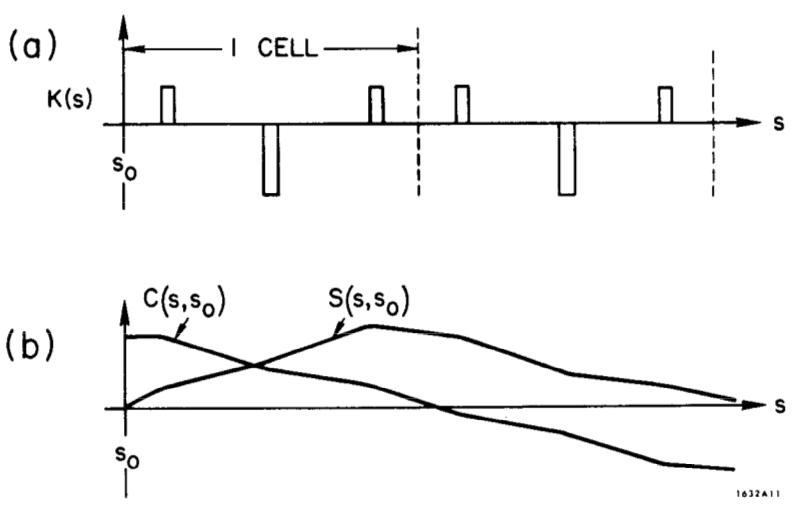
\includegraphics[width=0.7\linewidth]{./Figuras/fig11.jpeg}
	\caption{Focussing function $K(s)$ and two trajectories: the cosine-like trajectory and the sine-like trajectory for the starting azimuth $s_0$.}
	\label{fig:fig11}
\end{figure}

The detailed form of $C$ and of $S$ will depend on the reference azimuth $s_0$. They are in general, \textit{not} periodic functions, even though $K(s)$ is. For a ring with stable trajectories, $C$ and $S$ are bounded oscillatory functions which have a different shape on each successive revolution of the ring; although they are ``quasi-periodic'' in the sense that after some number of revolutions they will lie very close (or in some hypothetical cases even exactly on) the trajectory of an earlier revolution.

Now since Eq.~\eqref{eq:2.31} is linear in $x$, any linear combination of $C$ and $S$ will also describe a possible trajectory; and more particularly, all possible trajectories can be described by such a linear combination. That is, for any trajectory
\begin{align}
	x(s) &= C(s,s_0)x_0 + S(s,s_0)x_0'\\
	x'(s) &= C'(s,s_0)x_0 + S'(s,s_0)x_0'
\end{align}
where $C'$ and $S'$ are the derivations of $C$ and $S$ with respect to $s$; and $x_0$ and $x_0'$ are the values of $x$ and $x_0'$ at $s_0$.

It is often convenient to write the last two equations in a matrix notation. Let's let $\boldsymbol{x}(s)$ stand for the “vector” whose components are $x(s)$ and $x'(s)$;
\begin{align}
	\boldsymbol{x}(s) = \begin{bmatrix}
	x(s)\\
	x'(s)
	\end{bmatrix}
\end{align}
Then we may write that
\begin{align}
	\boldsymbol{x}(s)=\boldsymbol{M}(s,s_0)\boldsymbol{x}(s_0)
\end{align}
in which $\boldsymbol{M}$ is the transfer matrix to $s$ from $s_0$, which depends only on the properties of the guide field between the two azimuths. It's elements can be written in terms of the cosine-like and sine-like functions:
\begin{align}
	\boldsymbol{M}(s,s_0) = \begin{bmatrix}
	C(s,s_0) & S(s,s_0)\\
	C'(s,s_0) & S'(s,s_0)
	\end{bmatrix}\label{eq:2.37}
\end{align}
The transfer matrix for any span of $s$ can often be conveniently found in terms of the matrices for segments of the span, since for any $s_1$ between $s_0$ and $s$,
\begin{align}
	\boldsymbol{M}(s,s_0) = \boldsymbol{M}(s,s_1)\boldsymbol{M}(s_1,s_0)
\end{align}
The matrix for a segment which extends from $s_1$ to $s_2 = s_1 + \ell$ with a constant $K$ is given in Table~\ref{tab:tab1} for the three cases; $K > 0$, $K = 0$, and $K < 0$. They may be derived from the equations in \eqref{eq:2.32}.

The transfer matrix method is useful when designing a ring, or in looking at special problems such as the initial trajectories at injection. It does not, however, provide the most convenient description of the general nature of the trajectories of stored electrons. For many purposes another method of describing the trajectories is more useful. It may be called the ``pseudo-harmonic'' description.
\begin{table}[!ht]
	\caption{Transfer matrices for segments of constant $K$.}
	\centering
	\begin{tabular}{lrl}
		$K>0:$ & $\boldsymbol{M}(s_2,s_1) =$ &  $\begin{bmatrix}
			\cos(\sqrt{K}\ell) & \frac{1}{\sqrt{K}}\sin(\sqrt{K}\ell)\\
			-\sqrt{K}\sin(\sqrt{K}\ell) & \cos(\sqrt{K}\ell)
			\end{bmatrix}$\\
		\\
		$K=0$: & $\boldsymbol{M}(s_2,s_1) =$ & $\begin{bmatrix}
			1 & \ell\\
			0 & 1
			\end{bmatrix}$\\
		\\
		$K<0:$ & $\boldsymbol{M}(s_2,s_1) =$ & $\begin{bmatrix}
				\cosh(\sqrt{-K}\ell) & \frac{1}{\sqrt{-K}}\sinh(\sqrt{-K}\ell)\\
				\sqrt{-K}\sinh(\sqrt{-K}\ell) & \cosh(\sqrt{-K}\ell)
				\end{bmatrix}$
	\end{tabular}
	\label{tab:tab1}
\end{table}

The general solutions of Eq.~\eqref{eq:2.31} can be written as
\begin{align}
	x(s) = a\zeta(s)\ \cos\{\varphi(s)-\vartheta\}\label{eq:2.39}
\end{align}
where $\zeta(s)$ and $\varphi(s)$ are specially defined functions of $s$ with certain convenient properties and $a$ and $\vartheta$ are constants (``initial conditions'') which determine a particular trajectory. Specifically, if we define
\begin{align}
	\varphi(s) = \int_{0}^{s} \frac{d\bar{s}}{\zeta^2(\bar{s})}
\end{align}
so that
\begin{align}
	\varphi'(s) = \frac{1}{\zeta^2}
\end{align}
and if we define $\zeta(s)$ to be that positive valued, analytic function which satisfies
\begin{align}
	\zeta'' = -K(s)\zeta+\frac{1}{\zeta^3}\label{eq:2.42}
\end{align}
then, as you can show by direct substitution, the $x(s)$ of Eq.~\eqref{eq:2.39} satisfies the differential equation~\eqref{eq:2.31}. For a more rigorous approach, you can check the appendix, Section~\ref{sec:FloquetTheorem}.

Following tradition, I shall choose generally to deal rather than with $\zeta(s)$, with its square -- which is universally written as $\beta(s)$. With this translation Eq.~\eqref{eq:2.39} gets replaced by
\begin{align}
	x(s) = a\sqrt{\beta(s)}\ \cos\{\varphi(s)-\vartheta\}\label{eq:2.43}
\end{align}
with
\begin{align}
	\varphi(s) = \int_{0}^{s} \frac{d\bar{s}}{\beta(\bar{s})}\label{eq:2.44}
\end{align}
and
\begin{align}
	\beta(s) = \zeta^2(s)\label{eq:2.45}
\end{align}
so that $\sqrt{\beta(s)}$ is the function defined by Eq.~\eqref{eq:2.42}. Given the focusing function $K(s)$ for a storage ring, the function $\beta(s)$ is uniquely determined; it can therefore, serve as an alternate “representation” of the focusing characteristics of the ring. Notice, however, that while $K(s)$ is given in terms of the local properties (at each $s$) of the guide field, the function
$\beta(s)$ -- or $\zeta(s)$ -- depends on the total configuration of the ring. On the other hand once $\beta(s)$ is known, $K(s)$ can be immediately obtained from its local derivatives by Eqs. \eqref{eq:2.42} and \eqref{eq:2.45}. But it is $\beta(s)$ which reveals more directly the significant characteristics of the trajectories of stored electrons.

It is possible to have guide fields that do not result in stable (that is, bounded) trajectories. For such fields $\beta(s)$ is not defined. But such fields can hardly be said to form a ``storage'' ring; so we are not interested in them here. Although they may be of interest to the storage ring designer -- as something to be avoided!

I will return later to a discussion of how $\beta(s)$ is related to the guide field properties; but it will be more useful to look first at the qualities of the trajectories described by the pseudo-harmonic solutions described by Eq.~\ref{eq:2.43}.

Don't forget that all of the discussion of this section applies equally to vertical as well as to radial motion. A ring is therefore, described by the two functions $\beta_x$ and $\beta_y$ (or $\zeta_x$ and $\zeta_y$), which are derived from the two focussing functions $K_x$ and $K_y$. It follows that the phase function $\varphi(s)$ is also different for motion in $x$ and in $y$.
